\documentclass{article}

\usepackage{graphicx}
\usepackage{tikz}
\usepackage{tikzsymbols}
\usetikzlibrary{calc,patterns,shapes.geometric}
\pagestyle{empty}
\usepackage[margin=0pt]{geometry}
\geometry{papersize={14in,12in}}

\def\centerarc[#1](#2)(#3:#4:#5){\draw[#1] ($(#2)+({#5*cos(#3)},{#5*sin(#3)})$) arc (#3:#4:#5);}

\begin{document}
	\begin{figure}
		\centering
		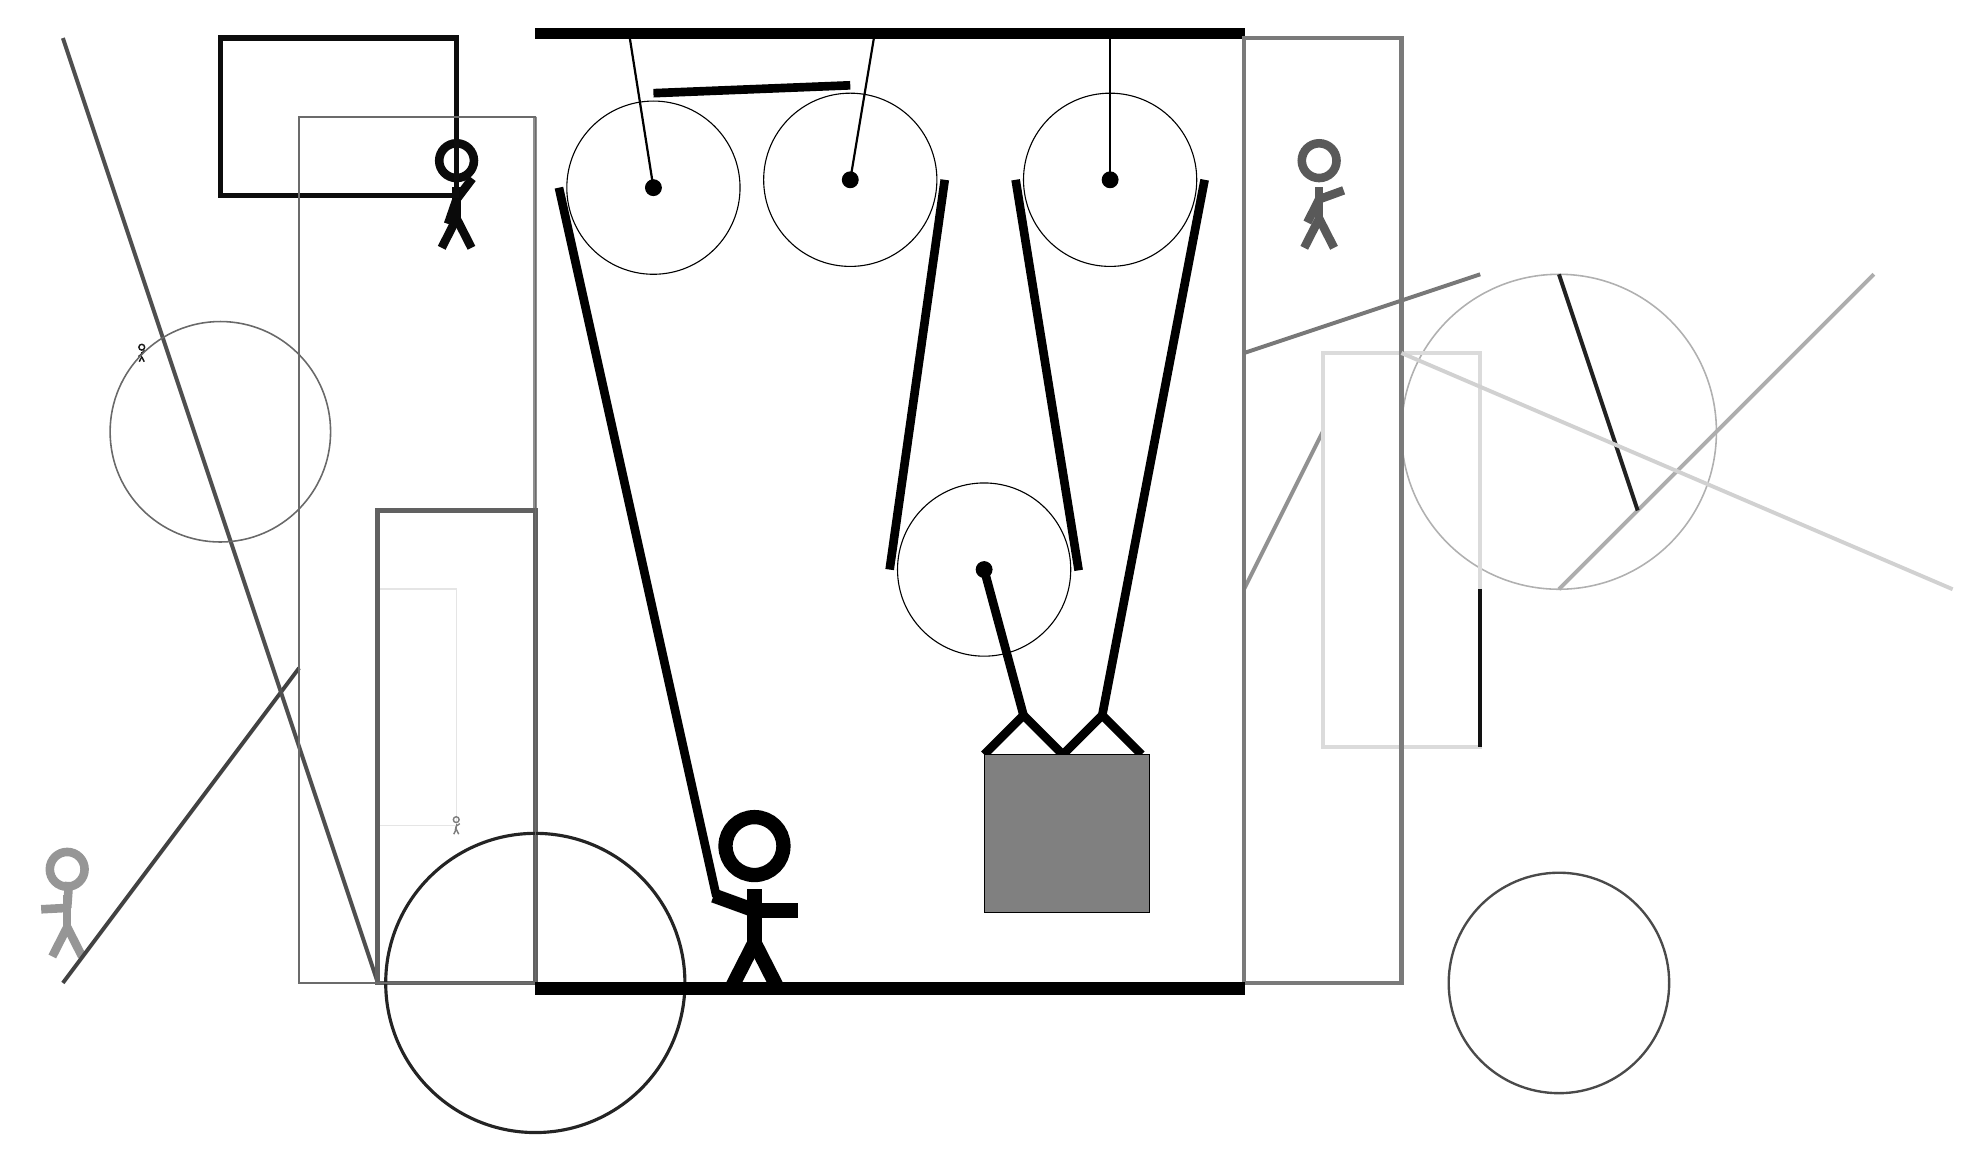
\begin{tikzpicture}
			%%%%% START %%%%%
			
			\draw[fill=black] (-3, 9) rectangle (6, 9.125);
			
			\draw (1, 7.2) circle (1.1);
			\draw[fill=black] (1, 7.2) circle (0.1);
			\draw[thick] (1, 7.2) -- (1.3, 9);
			
			\draw (4.3, 7.2) circle (1.1);
			\draw[fill=black] (4.3, 7.2) circle (0.1);
			\draw[thick] (4.3, 7.2) -- (4.3, 9);
			
			\draw (2.7, 2.25) circle (1.1);
			\draw[fill=black] (2.7, 2.25) circle (0.1);
			
			\draw[line width=1.1mm]  (2.7, -0.1) -- (3.2, 0.4) -- (3.7, -0.1) -- (4.2, 0.4) -- (4.7, -0.1);
			\draw[fill=black!50] (2.7, -0.1) rectangle (4.8, -2.1);
			
			\draw (-1.5, 7.1) circle (1.1);
			\draw[fill=black] (-1.5, 7.1) circle (0.1);
			\draw[thick] (-1.5, 7.1) -- (-1.8, 9);
			
			\draw [line width=0.2mm, color=black!31](10, 4) circle (2.0);
			
			\node[line width=0.4mm, color=black!41] at (-9, -2) {\Strichmaxerl[6][3][86]};
			\draw[line width=0.5mm, color=black!32](10, 2) -- (14, 6);
			\draw [line width=0.3mm, color=black!71](10, -3) circle (1.4);
			\node[line width=0.4mm, color=black!96] at (-4, 7) {\Strichmaxerl[6][71][53]};
			\draw[line width=0.5mm, color=black!74](-6, 1) -- (-9, -3);
			\draw[line width=0.5mm, color=black!19](-3, -3) -- (-5, -3);
			
			\draw[line width=0.7mm, color=black!95] (-4, 9) rectangle (-7, 7);
			\draw[line width=0.5mm, color=black!69](-5, -3) -- (-9, 9);
			\draw[line width=0.5mm, color=black!43](6, 2) -- (7, 4);
			
			\draw[line width=0.5mm, color=black!14] (7, 5) rectangle (9, 0);
			
			\node[line width=0.4mm, color=black!65] at (7, 7) {\Strichmaxerl[6][63][20]};
			\draw[line width=0.2mm, color=black!10] (-4, 2) rectangle (-5, -1);
			\draw[line width=0.5mm, color=black!87](11, 3) -- (10, 6);
			\draw[line width=0.5mm, color=black!44] (-3, -3) rectangle (-3, 8);
			\node[line width=0.3mm, color=black!90] at (-8, 5) {\Strichmaxerl[1][43][52]};
			
			\draw[line width=0.6mm, color=black!62] (-5, 3) rectangle (-3, -3);
			\draw [line width=0.4mm, color=black!86](-3, -3) circle (1.9);
			\draw[line width=0.2mm, color=black!58] (-3, 8) rectangle (-6, -3);
			\draw [line width=0.2mm, color=black!59](-7, 4) circle (1.4);
			\draw[line width=0.6mm, color=black!52] (8, -3) rectangle (6, 9);
			
			\draw[line width=0.5mm, color=black!53](6, 5) -- (9, 6);
			\draw[line width=0.5mm, color=black!18](8, 5) -- (15, 2);
			\node[line width=0.2mm, color=black!51] at (-4, -1) {\Strichmaxerl[1][77][34]};
			\draw[line width=0.5mm, color=black!93](9, 2) -- (9, 0);
			
			\draw[line width=1.1mm](-0.7, -1.9) --  (-2.7, 7.1);
			\centerarc[line width=1.1mm](-1.5, 7.1)(90:180:1.2000000000000002);
			\draw[line width=1.1mm](-1.5, 8.3) -- (1, 8.4);
			\centerarc[line width=1.1mm](1, 7.2)(0:90:1.2000000000000002);
			\draw[line width=1.1mm](2.2, 7.2) -- (1.5, 2.25);
			\centerarc[line width=1.1mm](2.7, 2.25)(180:370:1.2000000000000002);
			\draw[line width=1.1mm] (3.9, 2.24) -- (3.1, 7.2);
			\centerarc[line width=1.1mm](4.3, 7.2)(0:180:1.2000000000000002);
			\draw[line width=1.1mm](4.2, 0.4) -- (5.5, 7.2);
			\draw[line width=1.1mm] (3.2, 0.4) -- (2.7, 2.25);
			
			\node at (-0.2, -2) {\Strichmaxerl[10][-20][0]};
			
			\draw[fill=black] (-3, -3) rectangle (6, -3.15);
			
			%%%%% END %%%%%
		\end{tikzpicture}
	\end{figure}	
\end{document}